\subsection{The Third Marker}\label{sec:full_marker3}
The third marker, seen in figure \ref{marker:corny}, contains an image of packaging from a granola bar.
Here the colors are not distinct enough to use as the source and there is no good definable shapes in the image worth searching for.
In those situations can the Scale Invariant Feature Transform (SIFT) be used.

SIFT points can then be found on the marker and matched to the point found in the image.
Once the features are extracted, they can be inserted into a search tree using FLANN.
FLANN makes a balanced binary search tree so the features in the scene and the features in the marker can be matched.
Then the matches are compared using RANSAC and the corners of the marker is projected onto the image. 

To test if the marker is successfully detected, lines between the corners have been drawn onto the image.
In figure \ref{fig:sift_detection} can it be seen that the marker is successfully detected.

\begin{figure}[h]
 \centering
 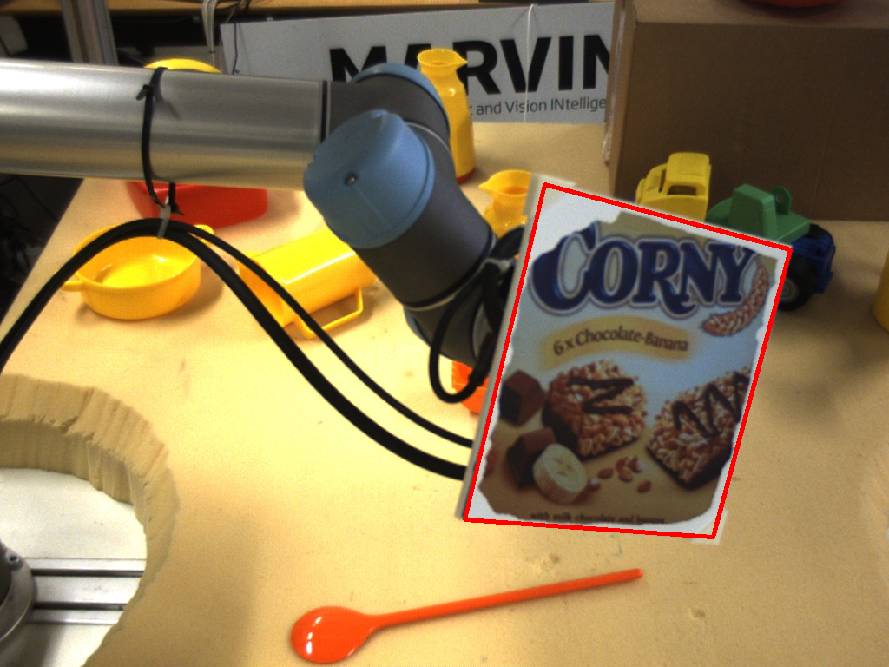
\includegraphics[width=\exampleWidth]{graphics/sift_detection}
 \caption{SIFT detection on an image.}
 \label{fig:sift_detection}
\end{figure}

Testing the performance of SIFT shows that it successfully detected 30/30 images on the easy set and 52/52 images on the hard set.
To measure the performance of SIFT, the timing was measured. 
The timing is shown in figure \ref{fig:time_sift_unoptimized}. 
The timing of calculating SIFT takes $665$ ms on average to detect the marker.
This can be a problem if a robot should react on a moving object.
The timing is split into three problems, the time it takes to find the keypoints, the descriptors and the homography.
The homography can be found faster by reducing the number of matches.
This could be done by removing matches that deviate from the minimum distance between two features.
Running with this optimization, the total time goes down to a $630$ ms on average.

\begin{figure}[h]
 \centering
 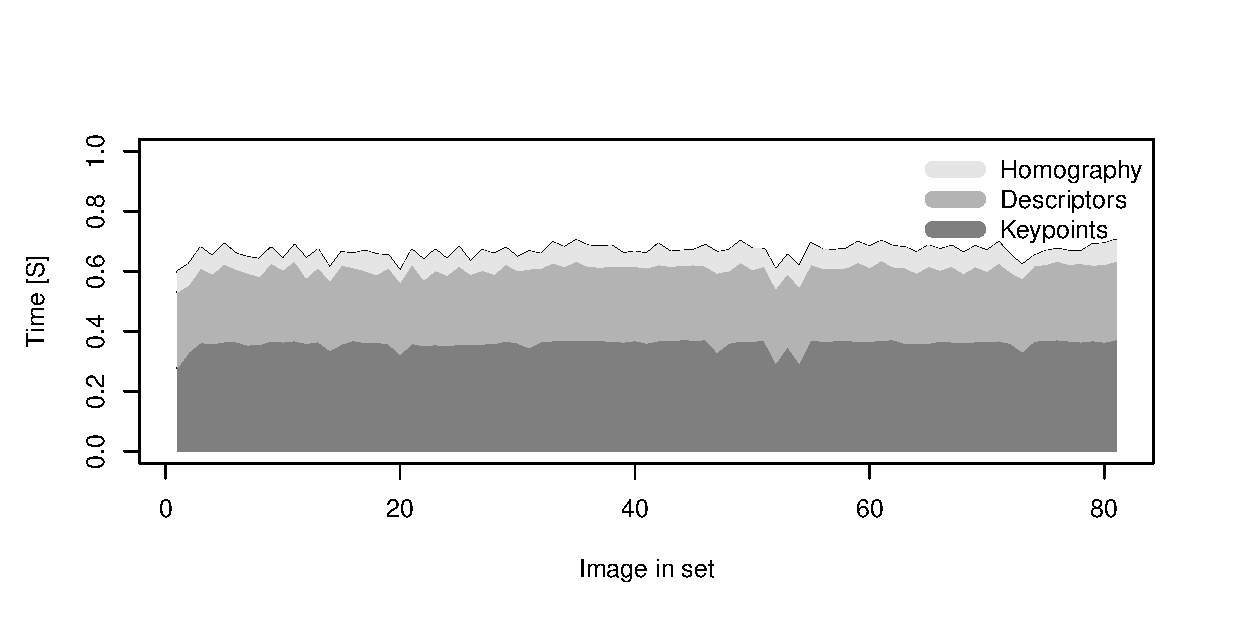
\includegraphics[width=\fullImageWidth]{graphics/marker3_timing_unoptimized}
 \caption{Timing for finding the marker with SIFT.}
 \label{fig:time_sift_unoptimized}
\end{figure}

%In figure \ref{fig:time_sift_unoptimized} it can be seen that calculating the SIFT features is what is taking the majority of the time.
In figure \ref{fig:time_sift_unoptimized} is the time taken to calculate the matches shown.
It can be seen that calculating the SIFT features is the dominant factor of the process.
A way to reduce this is to reduce the image by cropping.
Since the scenario is that the robot is tracking the marker, locality of the marker in the image can be used.
Since the distance to the object does not change drastically, the marker will keep the same size in relation to the image.
By using the last known position of the marker and cropping it, the time to find the SIFT features can be reduced.
If the marker is not found, as it would be the case if the marker has moved too far out of frame, the entire picture should be used for the next analysis.
This would also be the case for the first image, as the position starts as unknown.

In figure \ref{fig:time_sift_crop} is the time shown to find the marker using the cropping optimization.
The timing now has outliers as it takes more time to process the larger image.
The median is then found in order to estimate the time it takes to find the marker with the optimized solution.
The median is measured to be $272$ ms.
The large image is analyzed two times, once for the first image and once for image 28 as the transition from 26 to 27 is not continuous.
The transition from the easy image set to the hard image set is continuous enough so the detector finds the marker.
On images where the marker is not present, the detector could successfully reject all images.


\begin{figure}[h]
 \centering
 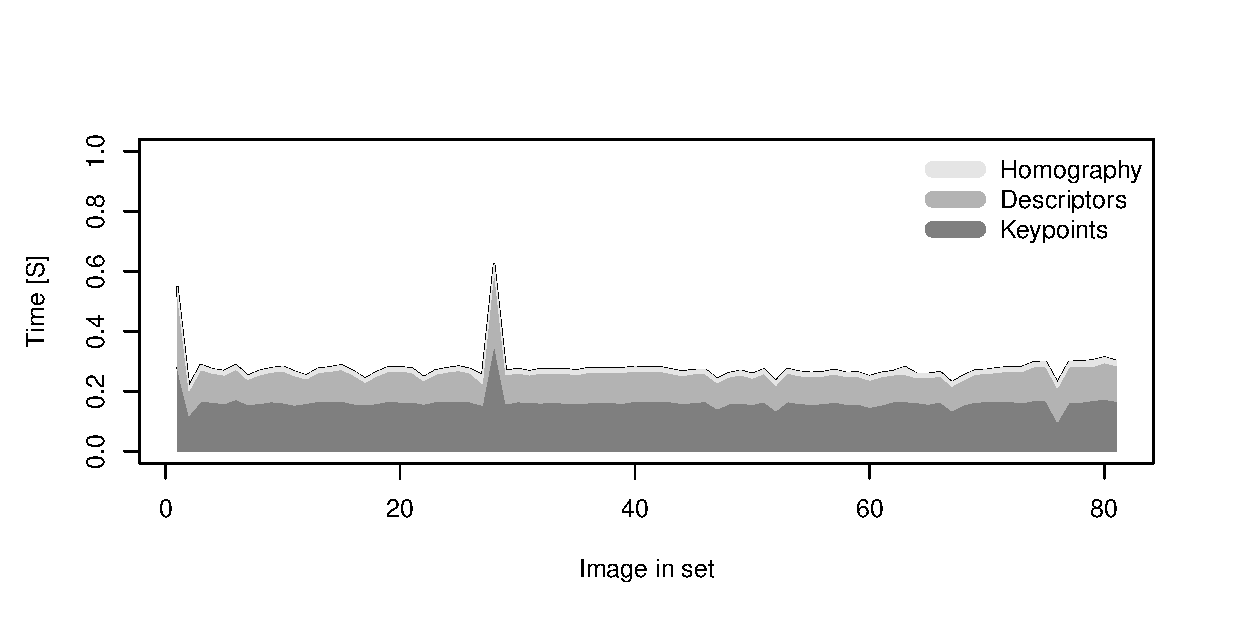
\includegraphics[width=\fullImageWidth]{graphics/marker3_timing_crop}
 \caption{Timing for finding the marker with SIFT optimized for servoing.}
 \label{fig:time_sift_crop}
\end{figure}

The four corner points of the rectangle are then returned as the points used for tracking.
